\section{Application Planning and Requirements}
\subsection{Requirements and Specifications}
In the next subsection, this thesis will present a brief discussion regarding the possible stakeholder requirements alongside a more detailed specification list from the development perspective.

The act of stock market prediction is usually incorporated in large financial applications which may offer a variety of functionalities. However, in those applications the core functionalities are considered of a higher importance and relevance than the actual reliability of the prediction. This application will try to incorporate some functionalities from generic financial applications, while maintaining its core to the actual prediction and useful information along in order to facilitate decisions for the users (investors).

The application has to be easily accessible and offer the users a friendly and familiar environment. The user should be able to select a list of favorite companies to follow. For each company, he should be able to check details about the company, check the historical price and check prediction on both historical and future data. Moreover, the user should be linked with some recent financial news which might affect the market or to run a simulation on a given interval of time on historical data with a fixed investment strategy. Lastly, in order to encourage user engagement and provide a good experience, a feedback platform is mandatory for improving further the development. 

\vspace{5mm}

From the development perspective we have decided a list of specifications which should be fulfilled by the application. The application will have a sign-up and login system, using two types of users: client and admin with different permissions. Further, we'll split the specification list in two based on the role.

\paragraph{Client User}
\begin{itemize}
    \item Register and login as an user
    \item List the available companies to follow
    \item List some recent news which might affect the future trend of the market
    \item Ability to select and add favorite companies
    \item Remove a company from your favorite list
    \item Request various details about a favorite company
    \item Request the historical data for a favorite company as a plot
    \item Request prediction for historical events to check the stability
    \item Request future prediction for the present moment for different time-horizons
    \item Run an investment simulation based on a set of companies and a fixed strategy
    \item Feedback report system to the developers
    \item Notification system regarding feedback answer
\end{itemize}

\paragraph{Admin User}
\begin{itemize}
    \item Login as an admin
    \item Create a new entity company with its details
    \item Update company details
    \item Update company networks links to make it available for the clients
    \item Remove a certain company from available companies for clients
    \item Respond to user feedback
    \item Request the system to update financial data available with new request from external API
\end{itemize}

\subsection{Application Architecture}
In order to facilitate accessibility for the application, the decided architecture is of type client-server where the client application will be a mobile application. This architecture was chosen with multiple reasons in mind while being known for its flexibility and allowing easily addition of different types of clients if necessary.

The need for a dedicated server (of sets of servers) stems firstly from the amount of financial data used for predictions. Bundling large amounts of data with a portable mobile application is unacceptable. Moreover, this data needs frequent updates from known sources which have free API-s available, but with some low limits of requests per day. In addition, a large amount of neural networks will be maintained for different goals, time-horizons and companies. While nowadays mobile phones are becoming more and more powerful being capable of running some machine learning tasks, still most of the work is done in the cloud on dedicated servers. Lastly, moving the computational cost from the client to a server allows the application to be run on a larger variety of devices which otherwise might have been insufficient.

In order to facilitate possible integration in modern cloud systems, we are going to split the server computation cost in two major parts. The first part which will directly communicate with the client application will contain the entire business logic necessary to address most features which do not require any sort of prediction. The second part will behave similar to a Cloud API service for machine-learning operations regarding stock market prediction. It will be standalone and totally separated from the first part, maintaining only the network architectures already trained and expose a REST API for the business logic server to request any computations regarding prediction. The following picture attached contains a visual description of what has been discussed.

\begin{figure}[H]
\centering
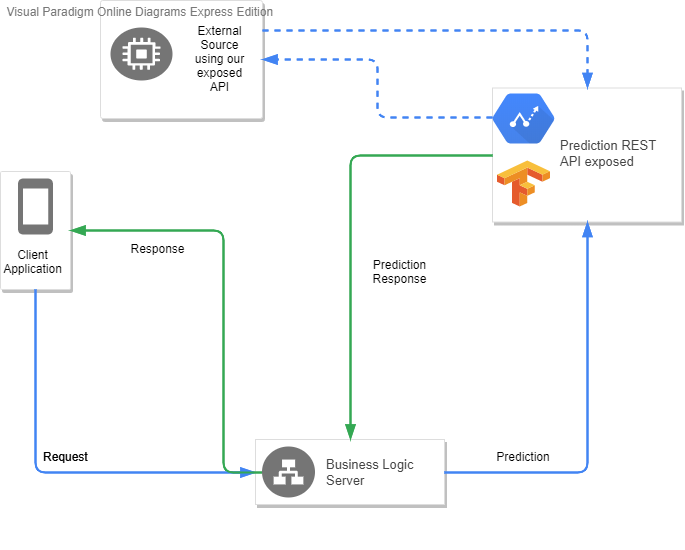
\includegraphics[height=12cm]{images/HighLevelArchitecture.png} 
\caption{High Level Architecture of the Application}
\label{fig:highlevelarchitecture}
\end{figure}


\subsection{Abstract Design - Use Case Diagram}
In the following subsection we are going to present the associated Use Case Diagram with the previously specified requirements specification. Two actors have been found along: the client and the admin. There are some use cases which belong to both, while most of them are separate.

\begin{figure}[H]
\centering
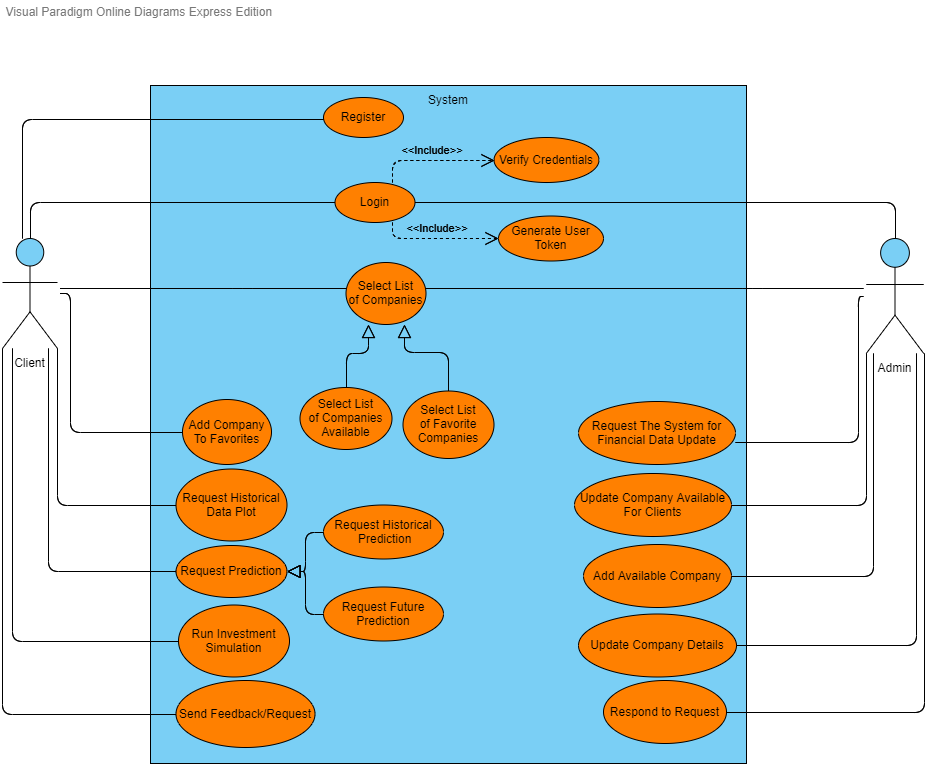
\includegraphics[height=13cm]{images/UseCaseDiagram.png} 
\caption{Use Case Diagram}
\label{fig:usecasediagram}
\end{figure}


\section{Application Design Phase}

\subsection{Exposed Prediction REST API}

\subsection{Business Logic Server}

As mentioned in the summary of application architecture, the main business logic will be maintained on a separate server  from the prediction API, offering more flexibility and reliability. As mentioned in the previous chapter, we are going to use the Spring Framework which offers a large variety of services such as inversion of control, Java Persistence API or testing.

We are going to work with a structured hierarchic layered structure borrowing elements from specific design patterns and strategies. In the past, the classic used for paradigm for creating a web/desktop application was a fully fledged Model-View-Controller (MVC) structure favoring a separation between layouts and components. However, since we are creating a separately client mobile app with its specific architecture, it is clear that the server will become a RESTful Web Services provider replacing the View layer with unique stateless HTTP requests between applications.

In order to maintain a degree of modularity we are going to obey the design principle of Separation of Concerns (SoC). This principle encourages the separation of different sections in an application such that each one is addressing a separate concern. While not ideally possible in the context of many applications, it offers some valuable guidelines in structuring to some degree the generic architecture of a program.

We will begin by splitting the business logic server design in two major blocks: core and web. Core will deal with most of the business logic required containing the persistence layer, the domain or the validation schema. On the other hand, the web block will deal with the exposed REST API maintaining different path patterns for different functionalities dependant on the client's role and mappings from and to the data transfer objects (DTOs) used. In terms of content for request and responses, we are going to adopt JSON (JavaScript Object Notation) as the standard data-interchange format opposed to older version such as XML.

Further, we are going to split the main blocks into separate layers to further address each concern. Each separate layer will translate in the implementation phase into at least one package separating the code for an improved visibility. The order will begin from the most external point with respect to receiving an HTTP Request and going down the hierarchy until reaching the persistence layer.

\begin{itemize}
    \item HTTP Filters Layer - before reaching the exposed REST API also known as the controller layer, each HTTP request should be filtered in order to assess its validity (URL, headers, content format). While the Spring Framework will deal with most of it automatically, we are still going to add some custom ones in order to address the security-login methodology or logging. More details will be found when talking specifically about the login functionality in detail
    \item Controller Layer - the main layer containing the mappings for request. This layer will communicate inside its web block with the others dependencies, while passing and retrieving data to the uppermost layer from the core block
    \item Data Transfer Objects Layer - it will cover the basic objects structures which are passed alongside the HTTP calls. It is used successfully in combination with the framework which is able to automatically convert back and forth JSON content and simple classes
    \item Mapping Layer - the mapping layer will include the converting logic between data transfer objects and the objects returned back by the core block separating this concern from the main controller layer above
    \item Service Layer - the uppermost and first layer of the core block. Its objective is to link the web block to the persistence and domain layers containing most of the primary business logic required using in addition a separate validation cover.
    \item Validation Layer - a relatively simple part of the core block responsible for validating the various inputs received from the client through the HTTP request absolving the service from this concern
    \item Domain Layer - contains the entities associated with the persistence layer representing the enterprise business model. In order to facilitate the Object Relational Mapping offered by the Spring Framework (via Hibernate), they include relevant relational mappings related to the database architecture
    \item Persistence Layer - offers a set of interface to ease the communication with the database by making use of the Java Persistence API (JPA) which is fully integrated in an extension of the Spring Framework
\end{itemize}

\begin{figure}[H]
\centering
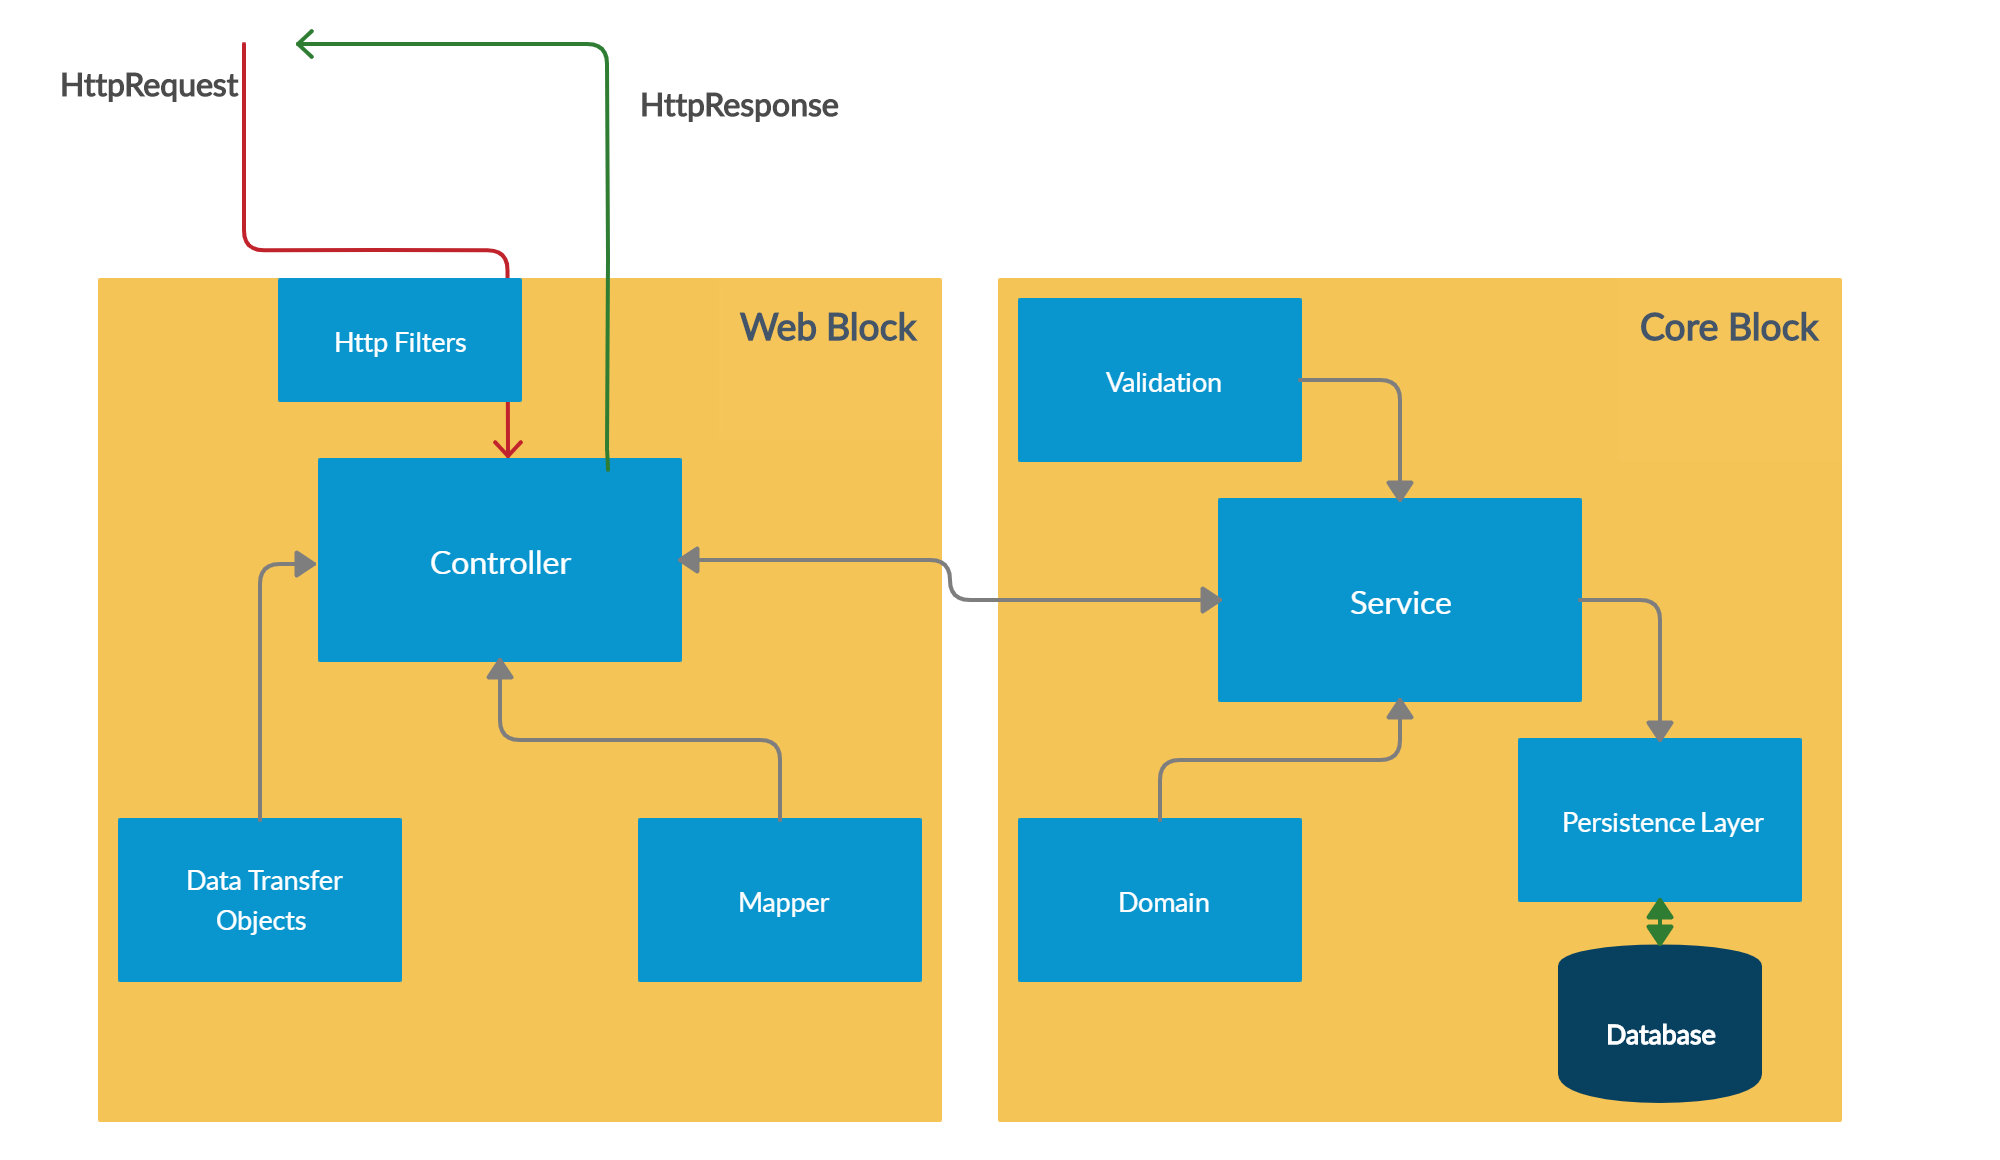
\includegraphics[height=11cm]{images/BusinessServerArchitecture.png} 
\caption{Business Server Logic Architecture}
\label{fig:businessserverarchitecture}
\end{figure}
\begin{flushright}
Created with: https://creately.com/
\end{flushright}




\subsection{Client Mobile Application}

\section{Application Core Functionalities}

\subsection{Login}
The first important functionality which is going to be implemented and tested is the login. In order to offer a personalized experience for each user, an account will be associated to each individual. However, since the API exposed from the business server will be available both for client and admin tasks, further methodologies should arise to differentiate and assure the security stability of the system.

The characteristics of the REST (Representational State Transfer) architectural style will influence the most. Because a request is basically stateless in this context, the server cannot understand by itself if some consecutive requests are from the same user or not. For this reason, we will implement token-based authentication system which is being used successfully in various systems with specialized authentication servers. We will not utilize in this case the official solution offered by the framework Spring Security in order to add more overhead to our application, while maintaining an open view about what is happening behind the scenes with each request.

In a token-based authentication system, the system must hold live information about the list of connected users and their minimal useful states. For this reason, a new class will be created called Session which will maintain the useful contents for a single connection. Consequently, the session will contain the connection token, the user ID for reducing business operations, the email associated with its account, a Boolean denoting whether the account has admin rights or not and finally a creation time in order to limit the availability time for a connection. In order to maintain fast retrieval for a session based on the token, the server will maintain an in-memory map containing a token as the key and the associated session as a value. Every time a new connection -login action will be successful- a new entry will be added in the map, while a logout or an expired request will be equivalent with removing that entry. From that moment, each subsequent request will contain the token as an 'Authorization' header attached.


\subsubsection{Implementation and Testing}

On the mobile side of the application, the login implementation involves several components. First, there is an associated LoginActivity which has linked a layout file containing the specific GUI page. The layout offers two fields similar to an authentication form for the email and the password, each offering an initial hint and an error message after typing until the content respects the pattern checked by a separate validator class. Besides the input fields, there is only one button for starting the login action to the server. From the moment it is pressed, the last front-end validation is checked again for the patterns. If the validation passes, a new coroutine scope is created to handle the computational cost outside the UI thread. Inside the coroutine scope, a network service class is called in order to request the server for a new connection. If the request is was successful, the token will be stored at the application level and the main client activity will be opened. Otherwise, an error message will be displayed in the user interface.


\begin{figure}[H]
\centering
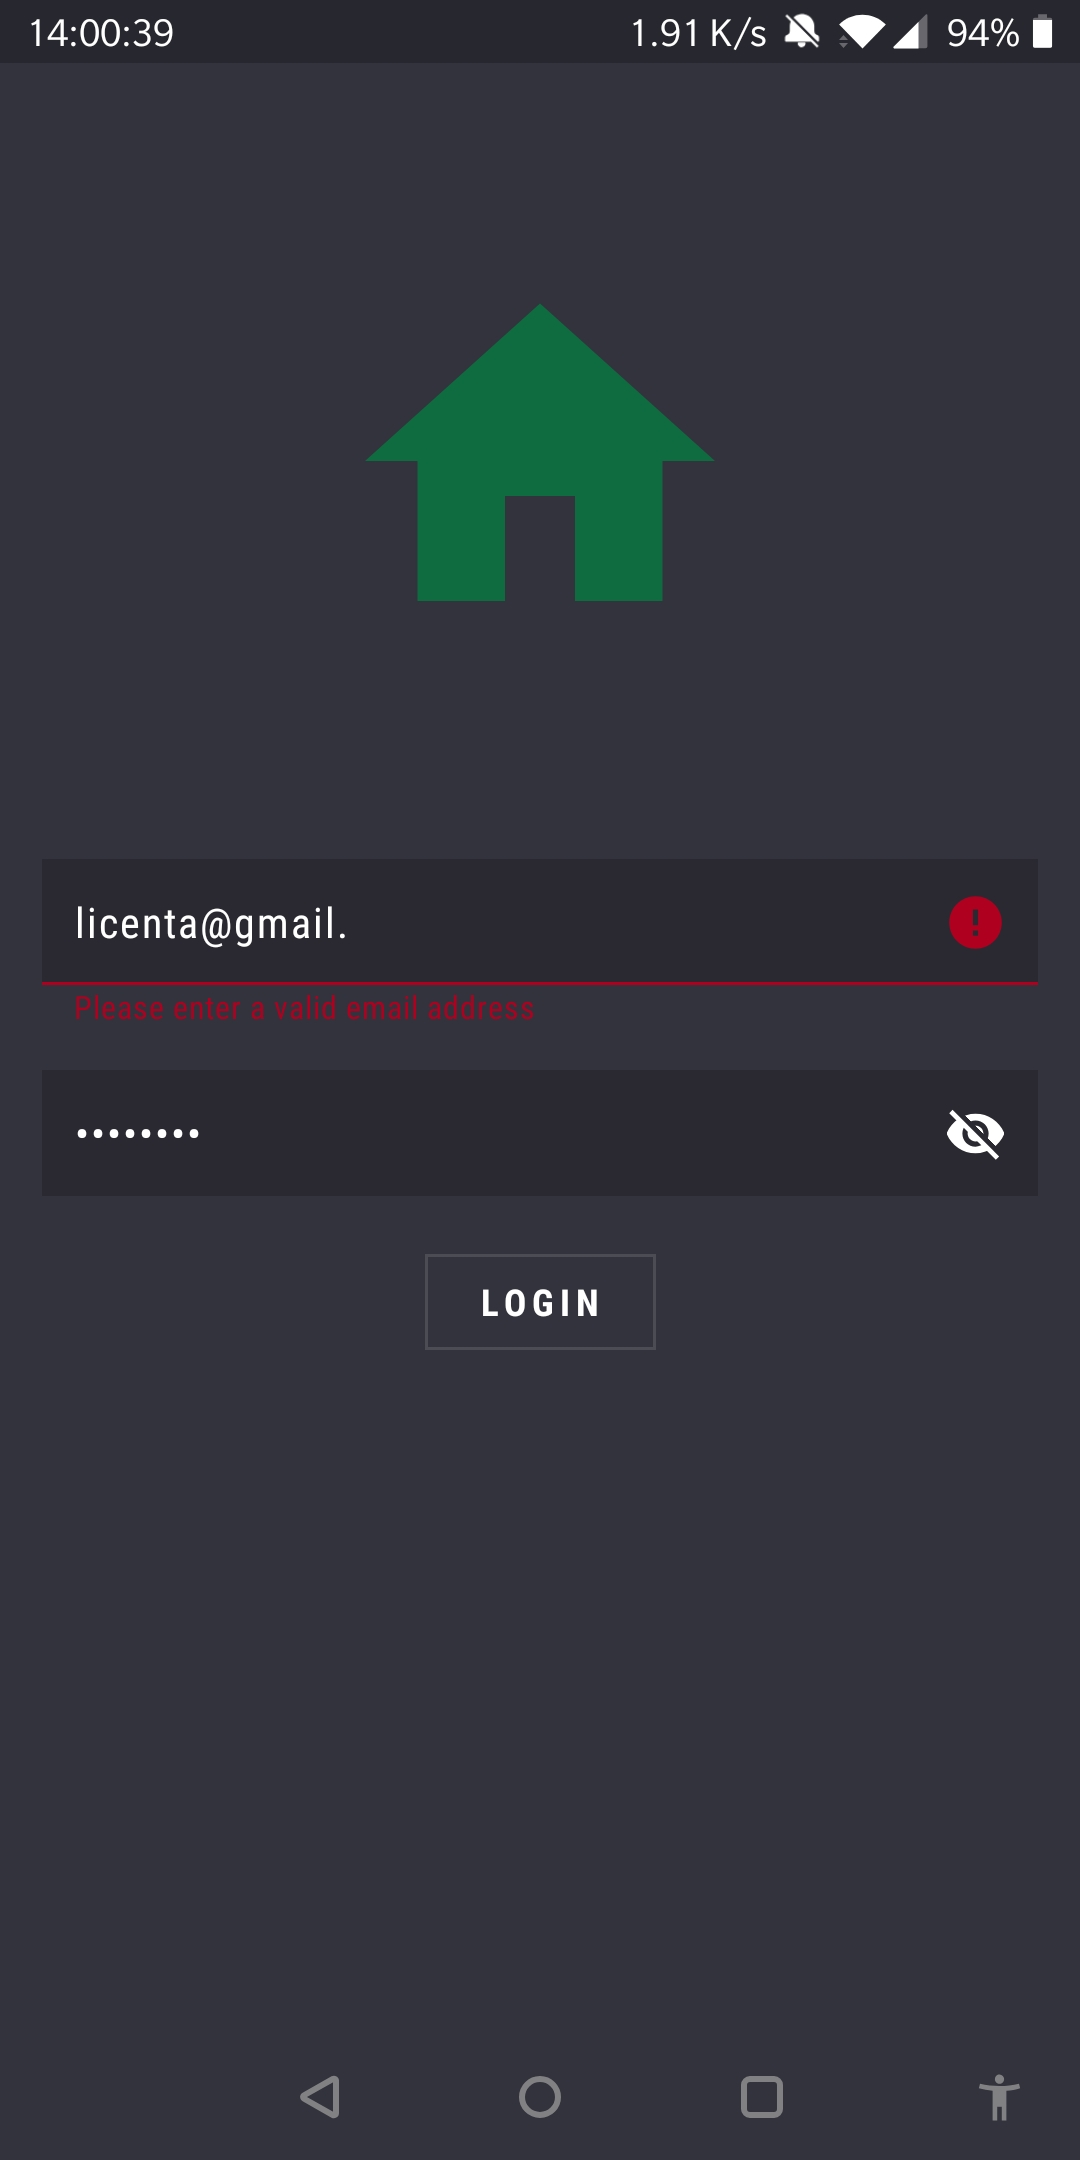
\includegraphics[height=10cm]{images/LoginGUIScreenshot.jpg} 
\caption{Login GUI Screenshot}
\label{fig:loginguiscreenshot}
\end{figure}

On the server side, the specific login request passed initially through only one basic logging HTTP filter. It reaches the LoginController which will pass the request further along to the core block which will check whether the account combination exists or not. If the request is valid, a new session object is created with its associated token which will be passed back to the web block. Otherwise, an exception is thrown with the according error message which will be called, logged and passed back in the HTTP Response. From this moment, the client will be responsible to hold the token in a private space and pass it along as an 'Authorization' to every subsequent request. Every other request will have a specific URL pattern which will be filtered by the other necessary HTTP filters.

Each server-side HTTP filter is inheriting from GenericFilterBean which is a component offered by the Spring Framework to specify more easily the necessary behaviour. Behind the scenes the base class for filtering is the old Filter interface proposed by the Java Servlet library. Each class must override a single method called doFilter() which is receiving the request and the response as parameters and is implementing the business logic along the filter chain. In order to specify specific parameters for our filter such as the order of execution, the URL patterns and such, each class should be associated to an unique FilterRegistrationBean which will inform the framework how and when to instantiate and arrange them.

In terms of testing, we are going to test at two different layer levels while incorporating both unit and integration testing. Firstly, a set of tests will be created at the persistence layer with the help of data JPA tests from the framework. These tests will assess the quality of basic database operations such as finding the user with a specific email. Because we want to maintain our official MYSQL database in a stable state, the framework helps us by creating for each suite of tests an in-memory database (H2) which allows for fast computations and total isolation from the production database. Secondly, we will have a set of tests at the controller layer while incorporating mock objects for the core block. Consequently, we can unit test the controller layer while making sure that the HTTP request respect and follow the desired structured. Lastly, we will add integration testing by incorporating all the layers along our server, while maintaining the observation from the first set that the database used will not coincide with the production database.